\documentclass[varwidth=20cm,margin=1in,12pt]{standalone}
\usepackage{amsmath}
\usepackage{amssymb}
\usepackage{amsfonts}
\usepackage{graphicx}
\usepackage[russian]{babel}

\begin{document}

Адриан Москера К.\hfill группа: Б9121-02.03.01сцт\\

\begin{figure*}[t]
    \centering
    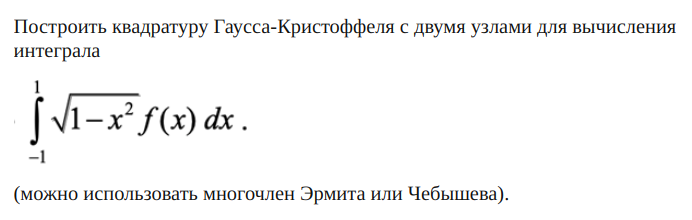
\includegraphics[width=18cm]{question.png}
\end{figure*}

\begin{align*}
    \int_{-1}^{1} \sqrt{1-x^2}f(x)dx
     & = \sum_{i=1}^{n} w_i f(x_i)                                                          \\
     & = \sum_{i=1}^{n} \frac{\pi}{n+1} \sin^2\left(\frac{i}{n+1}\pi\right)
    f\left(\cos\left(\frac{i}{n+1}\pi\right)\right)                                         \\
     & = \sum_{i=1}^{2} \frac{\pi}{3} \sin^2\left(\frac{i}{3}\pi\right)
    f\left(\cos\left(\frac{i}{3}\pi\right)\right)                                           \\
     & = \frac{\pi}{3} \sin^2\left(\frac{1}{3}\pi\right)
    f\left(\cos\left(\frac{1}{3}\pi\right)\right) +
    \frac{\pi}{3} \sin^2\left(\frac{2}{3}\pi\right)
    f\left(\cos\left(\frac{2}{3}\pi\right)\right)                                           \\
     & = \frac{\pi}{4} f\left(\frac{1}{2}\right) + \frac{\pi}{4} f\left(-\frac{1}{2}\right) \\
     & = \frac{\pi}{4} \left(f\left(\frac{1}{2}\right) + f\left(-\frac{1}{2}\right)\right)  \\
\end{align*}

\end{document}
